
% Computational Biology
% Introduction to Computational Biology
% 2022/2023
%  1. Introduction (max 1 page) [Motivation, background]
% 2. Methods (max 2 page)
% [Description on the theory and algorithms]
% 3. Datasets (max 0.5 page) [Applicability, what type of data]
% Report Template
% (maximum 10 pages ~ 5000 words)
% 4. Results (max 6 pages)
% [I) Describe Authors’ results. II) Test the program yourself: 1) Evaluate the performance, scalability, parallelization potential, server implementation viability, etc.; 2) report positive and negative aspects (e.g., ususer-friendliness); 3) test on new data, if possible]
% 5. Conclusions (max 0.5 page) [Final comments]

% Paper
% Link: https://academic.oup.com/bioinformatics/article/25/19/2607/180881?login=true
% Title: ShortRead: a bioconductor package for input, quality assessment and exploration of high-throughput sequence data
% Authors: Martin Morgan, Simon Anders, Michael Lawrence, Patrick Aboyoun, Hervé Pagès, Robert Gentleman
% Journal: Bioinformatics
% Year: 2009
% Volume: 25
% Issue: 19
% Pages: 2607-2608
% DOI: 10.1093/bioinformatics/btp450


\documentclass[12pt]{article}
\usepackage{authblk}
\usepackage{url}
\usepackage{graphicx}



%Title
\title{ShortRead R Package Report, for Computational Biology 2022/2023}

% Date 14/10/2022
\date{14 October 2022}

% Multiple authors
\author[1]{L. Ganser}
\author[2]{M. Fernandes}
\author[2]{R. Moreira}
\author[2]{V. Dalovic}
\affil[1]{École Polytechnique Fédérale de Lausanne, Switzerland}
\affil[2]{Instituto Superior T\'ecnico, Universidade de Lisboa, Portugal}

% Document
\begin{document}
\maketitle


\section{Abstract} 

The ShortRead R package is a collection of functions for reading and manipulating short-read sequencing data. It is designed to be used in conjunction with the Bioconductor project. The package provides a unified interface to read data from a variety of sequencing platforms, including Illumina, 454, SOLiD, and Ion Torrent. It also provides functions for quality control, trimming, and filtering of reads. The package also provides functions for mapping reads to a reference genome, and for variant calling. The package is available on CRAN and Bioconductor.
In this report, we explored the package while referring to %\cite{morgan2009}

\section{Introduction}
ShortReads is an R package that provides a unified interface to read data from a variety of sequencing platforms, including 
Illumina, 454, SOLiD, and Ion Torrent. It also provides functions for quality control, trimming, and filtering of reads.
The package also provides functions for mapping reads to a reference genome, and for variant calling. The package is available on CRAN and Bioconductor.


\subsection{Motivation}
ShortReads is a very used package and important for the Bioconductor project. It is used in many other packages and it is important to understand how it works.
We decided to explore this package to learn more about it and to be able to use it in the future.

\subsection{Background}
ShortReads is an R package that provides a unified interface to read data from a variety of sequencing platforms, including Illumina, 454, SOLiD, and Ion Torrent.
It also provides functions for quality control, trimming, and filtering of reads. The package also provides functions for mapping reads to a reference genome, and for variant calling. The package is available on CRAN and Bioconductor.

% Phred Score
\subsubsection{Phred Score}
Phred score is a way to represent the probability of a base being wrong.
It is used in the FASTQ format to represent the quality of a base. The Phred score is calculated as $-10 \log_{10} P$, where $P$ is the probability of the base being wrong. The Phred score is an integer between 0 and 40. The higher the Phred score, the higher the probability of the base being wrong. The Phred score is represented by the ASCII character with the same value as the Phred score plus 33. For example, the Phred score 40 is represented by the ASCII character '!'. The Phred score is also represented by the ASCII character with the same value as the Phred score plus 64. For example, the Phred score 40 is represented by the ASCII character '@'.

% FASTQ format
\subsubsection{FASTQ format}
The FASTQ format is a text-based format for storing both a biological sequence and its corresponding quality scores.
It is a text-based format for storing both a biological sequence and its corresponding quality scores. 
Each record contains four lines: the first line starts with a '@' character and is followed by a sequence identifier and an optional description (like a FASTA title line); the second line is the raw sequence letters; the third line starts with a '+' character and is optionally followed by the same sequence identifier (and any description) again; and the fourth line encodes the quality values for the sequence in Line 2, and must contain the same number of symbols as letters in the sequence. The quality values are encoded using the Phred quality score plus 33. For example, a base with a quality score of 40 has a character '!' as its quality value. The quality values are also encoded using the Phred quality score plus 64. For example, a base with a quality score of 40 has a character '@' as its quality value.

% FASTA format
\subsubsection{FASTA format}
The FASTA format is a text-based format for representing either nucleotide sequences or peptide sequences, in which nucleotides or amino acids are represented using single-letter codes.
The format is designed so that the file is human-readable, and can be parsed by software. The first line of the file must begin with a '>', which is followed by the sequence identifier and an optional description.
The sequence identifier and the description are separated by one or more spaces or tabs. The description is not used by most software. The second line contains the first line of the sequence. The sequence lines may be of any length.
The sequence ends when the next line begins with a '>'. The FASTA format is used in the ShortReads package to represent the reference genome.

\section{Methods}
To analyze the package, we looked into the Github repository\cite{shortreadsgit} and the documentation\cite{shortreadsdoc}.
We also used the RStudio IDE to run the examples and to test the package.
We will now analyze the following functions:
\begin{itemize}
    \item readFastq — Reads a FASTQ file and returns a \texttt{ShortRead} object.
    \item qa — Quality assessment of a \texttt{ShortRead} object.
    \item srFilter — Filters a \texttt{ShortRead} object. Pre-defined and bespoke filters are available.  
\end{itemize}


\subsection{The readFastq function and the ShortReadQ class}
The \texttt{readFastq} function reads a FASTQ file and returns a \texttt{ShortReadQ} R object,
a compact internal representation of the sequences. The \texttt{ShortReadQ} class inherits from the \texttt{ShortRead} class and adds the quality scores to the sequences.
The \texttt{ShortRead} class (see \texttt{AllClasses.R}) contains the following elements:
\begin{itemize}
    \item \texttt{sread} — A character vector containing the sequences.
    \item \texttt{id} — ?A character vector containing the sequence identifiers.?
\end{itemize}

The \texttt{ShortReadQ} class (see \texttt{AllClasses.R}) inherits from the \texttt{ShortRead} class and adds the quality scores to the sequences which are represented in a character vector.
The \texttt{readFastq} function (see \texttt{methods-ShortReadQ.R}) has the following arguments:
\begin{itemize}
    \item \texttt{dirPath} (Character vector) — The path to the directory containing the FASTQ files.
    \item \texttt{pattern} — The pattern describing the FASTQ file names to be read. Default is \texttt{"*.fastq"}, which results in line counts for all FASTQ files in the directory.
\end{itemize}

The \texttt{readFastq} function (see \texttt{methods-ShortReadQ.R}) has the following steps:
\begin{enumerate}
    \item The function searches for the FASTQ files in the directory specified by the \texttt{dirPath} argument matching the pattern specified by the \texttt{pattern} argument.
    \item If no FASTQ files are found, the function throws an error.
    \item The function reads elements using the \texttt{.read\_solexa\_fastq} function (?see \texttt{methods-ShortReadQ.R}?) and creates a \texttt{ShortReadQ} object.
\end{enumerate}



\subsection{Installation}
The ShortReads package can be installed from CRAN or Bioconductor. To install the package from CRAN, run the following command in R:
\begin{verbatim}
install.packages("ShortRead")
\end{verbatim}
To install the package from Bioconductor, run the following command in R:
\begin{verbatim}
if (!requireNamespace("BiocManager", quietly = TRUE))
    install.packages("BiocManager")
BiocManager::install("ShortRead")
\end{verbatim}

\subsection{Usage}
The ShortReads package provides a unified interface to read data from a variety of sequencing platforms,
including Illumina, 454, SOLiD, and Ion Torrent.
It also provides functions for quality control, trimming, and filtering of reads.
The package also provides functions for mapping reads to a reference genome, and for variant calling.
The package is available on CRAN and Bioconductor.

\subsubsection{Reads}
The ShortReads package provides a unified interface to read data from a variety of sequencing platforms, including Illumina, 454, SOLiD, and Ion Torrent.

\subsubsection{Quality Control}
The ShortReads package provides functions for quality control, trimming, and filtering of reads.

\subsubsection{Mapping}
The ShortReads package provides functions for mapping reads to a reference genome.

\subsubsection{Variant Calling}
The ShortReads package provides functions for variant calling.

\section{Results}
\subsection{The readFastq function}


\subsection{Evolution of the package over time}
\begin{figure}[h]
    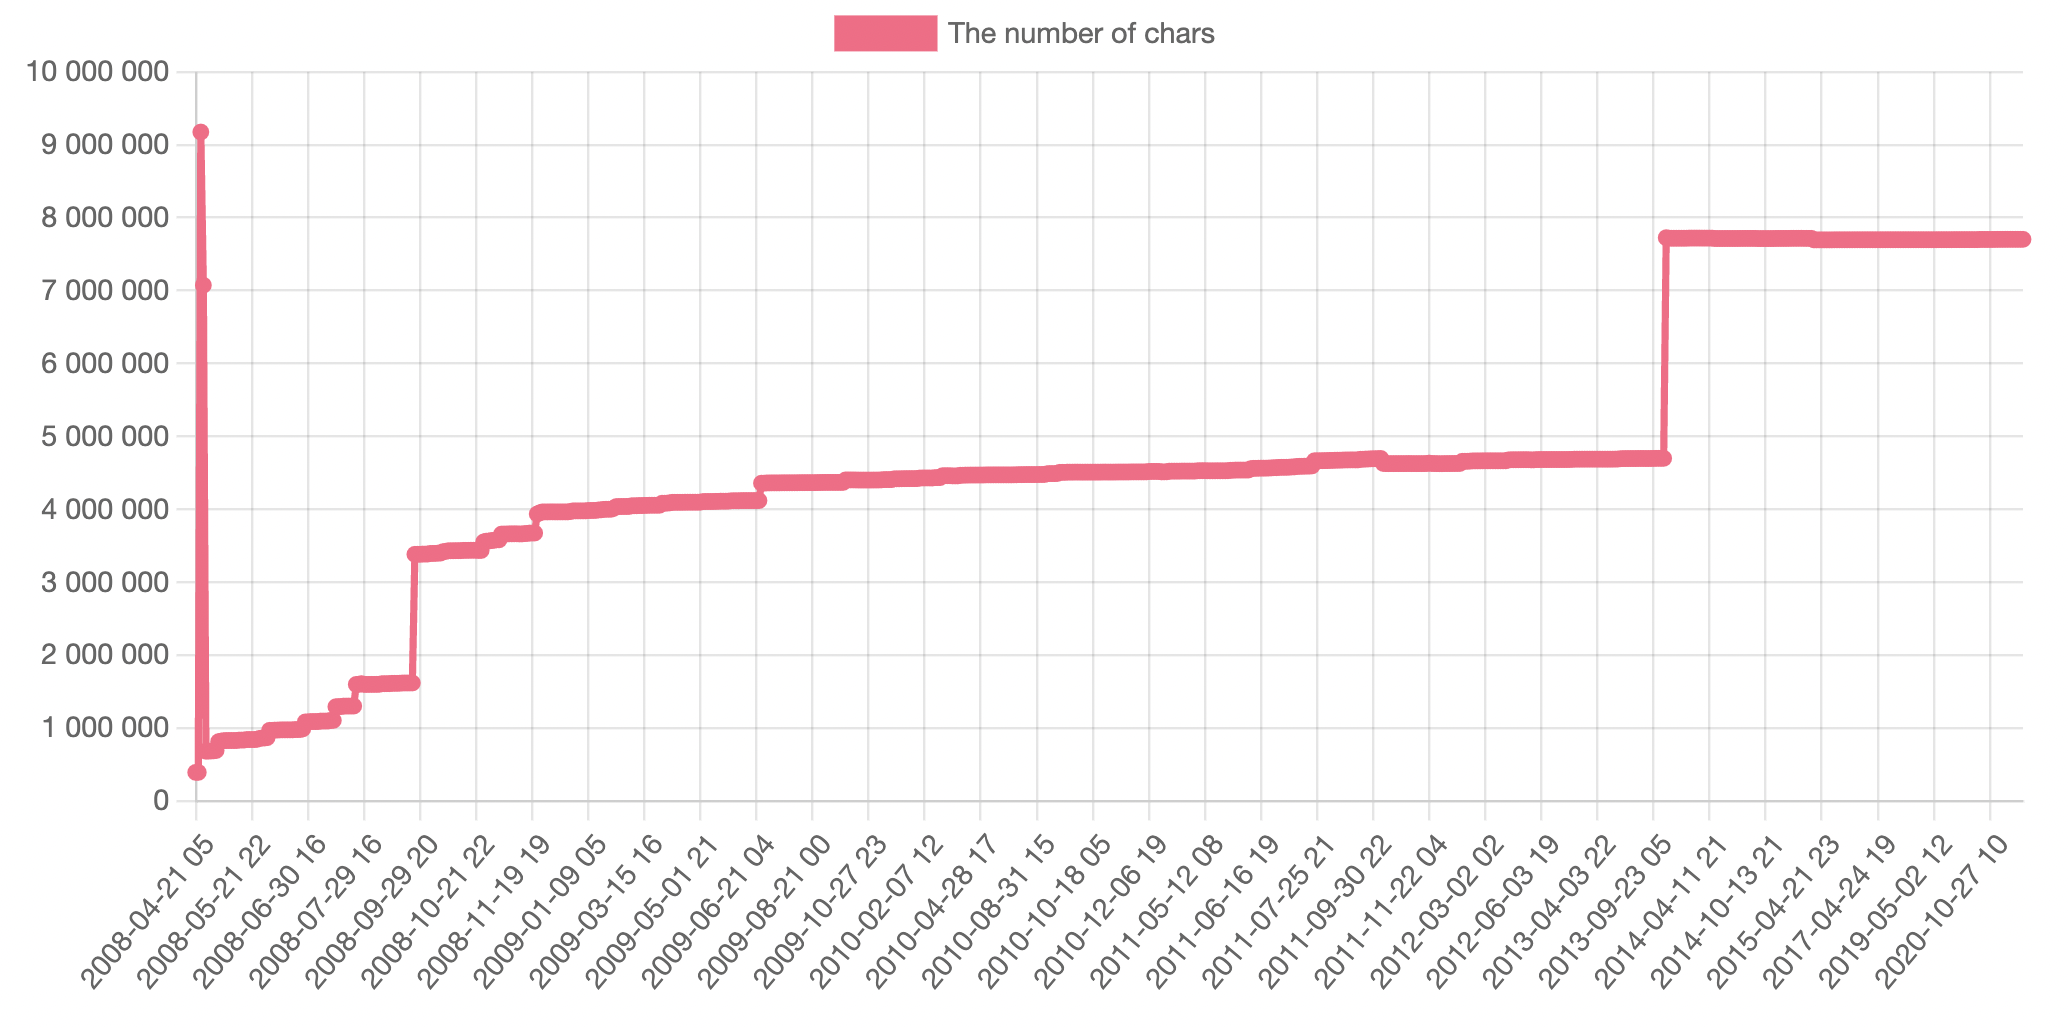
\includegraphics[width=0.8\textwidth]{figures/commits.png}
    \caption{Number of commits per month. Created using Writer-Stock %(文字数の推移),
    by PenguinCabinet}
    \label{fig:commits}
\end{figure}

The package was first added to Bioconductor in version BioC 2.3 (R-2.8) in 2008.
The first commit on Github was made in April 2008. The package has been updated regularly since then. The number of commits per month is shown in Figure \ref{fig:commits}.



% Bibliography
\begin{thebibliography}{10}
\bibitem{shortreadsgit}
ShortReads on Github.
\newblock \url{https://github.com/Bioconductor/ShortRead}
\bibitem{shortreadsdoc}
ShortReads documentation.
\newblock \url{https://bioconductor.org/packages/release/bioc/vignettes/ShortRead/inst/doc/ShortRead.pdf}
\bibitem{morgan2009}
Morgan, M.~T., et al. (2009).
\newblock Shortread: an r/bioconductor package for input, quality control, and
  preprocessing of short read sequence data.
\newblock \emph{Bioinformatics}, 25(16):2078--2079.
\end{thebibliography}


\end{document}
